Cinq points distincts de la grille plane sont choisis. Prouvez que vous pouvez
toujours en choisir deux tels que le segment reliant ces points passe par un
autre point de la grille. (Les points de la grille sont ceux qui ont des
coordonnées entières.)

\begin{center}
\resizebox{0.8\linewidth}{!}{%
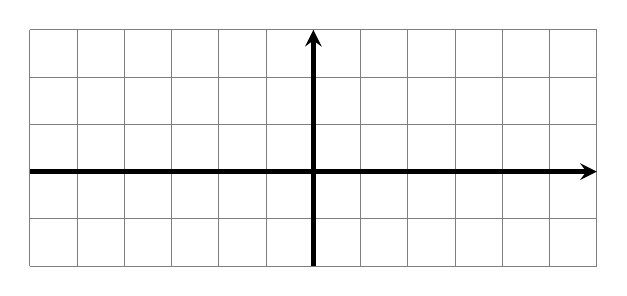
\begin{tikzpicture}[scale=.6, >=stealth]
  \draw[opacity=.5] (-6,-2) grid (6,3);
  \draw[ultra thick, ->] (-6,0) -- (6,0);
  \draw[ultra thick, ->] (0,-2) -- (0,3);
\end{tikzpicture}}
\end{center}
